%\documentclass[CJKutf8, table, handout]{beamer}
\documentclass[CJKutf8, table]{beamer}

%%%% theme used %%%%

\usetheme{Frankfurt}

%%%% import package %%%%
\usepackage{tikz}
\usepackage{CJKutf8}
\usepackage{graphicx}
\usepackage{pgf, pgfarrows, pgfnodes, pgfautomata, pgfheaps}
\usepackage{fancybox}
\usepackage{listings}
\usepackage{color}
\usepackage{caption}
\usepackage{hyperref}
\usepackage{textcomp}
\usepackage{enumerate}
\usepackage{courier}
\usepackage{listings}
\usepackage{tabularx}
\usepackage{wasysym}
\useoutertheme{progressbar}

\definecolor{listinggray}{gray}{0.9}
\definecolor{lbcolor}{rgb}{0.9,0.9,0.9}

\let\definition\relax
\newtheorem{definition}[theorem]{定义}
\lstset{
	language=Java,
	captionpos=b,
	tabsize=4,
	frame=lines,
	keywordstyle=\color{blue},
	commentstyle=\color{darkgreen},
	stringstyle=\color{red},
	breaklines=true,
	showstringspaces=false,
	basicstyle=\footnotesize,
	emph={label}
	}

%\pgfdeclareimage[height=60pt]{logo}{ictlogo.png}
%\logo{\pgfuseimage{logo}\hspace{-2pt}\vspace{-8pt}}

\usetikzlibrary{backgrounds}

\logo{
\includegraphics[height=0.045\textwidth]{ictlogo.png}}

%%%% title page %%%%

\title[Weibo-Mining]{基于微博短文本特征词扩展与降维技术的\\网络热点分析}
\subtitle{}
\author[Fu H.P.]{傅海平\inst{1} \and 赵震\inst{2} \and 崔遥\inst{3} 
\and 王维\inst{4} \and 王宁宁\inst{5} \and 马苗\inst{6}}
\institute[ICT]{\textsc{\inst{1,2,3,4}计算技术研究所, \inst{5}科技政策与管理研究所, \inst{6}国家空间科学中心\\[5ex]}
\textbf{中国科学院研究生院, 北京海淀, 中国\\[3ex]}
\texttt{\{\inst{1}haiping.ict, \inst{2}applelease, \inst{4}wangwei881116\}@gmail.com,
\\[1ex]\inst{3}cuiyao163@163.com,\\[1ex]\{\inst{5}578102899, \inst{6}550208974\}@qq.com}}
%\texttt{haipingf@gmail.com}
\date{\today}

% \AtBeginSection[]
% {
% \begin{frame}
%   \frametitle{Outline}
%   \tableofcontents[currentsection, currentsubsection, current]
% \end{frame}
% }

\AtBeginSection[]
{
\begin{frame}[shrink]
\begin{CJK}{UTF8}{gbsn}

	\frametitle{目录}
	\tableofcontents[%
 		currentsection, % causes all sections but the current to be shown in a semi-transparent way.
% 		currentsubsection, % causes all subsections but the current subsection in the current section to ...
% 		hideallsubsections, % causes all subsections to be hidden.
 		hideothersubsections, % causes the subsections of sections other than the current one to be hidden.
% 		part=, % part number causes the table of contents of part part number to be shown
%		pausesections, % causes a \pause command to be issued before each section. This is useful if you
% 		pausesubsections, %  causes a \pause command to be issued before each subsection.
% 		sections={ overlay specification },
	]
\end{CJK}
\end{frame}
}

%%%% begin document %%%%
\begin{document}

\begin{CJK}{UTF8}{gbsn}

\begin{frame}
\begin{CJK}{UTF8}{gbsn}
  \titlepage
\end{CJK}
\end{frame}

%%%%%%%%%%% 背景及目的 %%%%%%%%%%%%%%
\section{背景及目的}
\subsection{网络热点发现的兴起}
\begin{frame}
  \frametitle{Web2.0~时代的网络与个人}
  \begin{block}{}
    \begin{tiny}
      Web2.0~时代以个人为主导的网络传播兴起是互联网发展最显著的一个成果,可以将其视为个人传播时代正式到来的标志。
      个人媒体一定程度上引领了传统新闻媒介忽视的公共领域,并因其社会功能带来了不可忽视的影响。
      个人媒体不仅是个人话语、知识和思想的工具,更在结构一种新的社会、社会关系和社会资源。
    \end{tiny}
  \end{block}
  \pause
  \begin{block}{}
    \begin{tiny}
      \alert{微博},即微博客(MicroBlog)的简称,是一个基于用户关系的信息分享、传播以及获取平台,
      用户可以通过WEB、WAP以及各种客户端组建个人社区,以140字左右的文字更新信息,并实现即时分享。
    \end{tiny}
  \end{block}
  \pause
  \begin{definition}{微博}
    \begin{tiny}
      国内学者给出了微博的定义:微博是一种通过关注机制分享简短实时信息的广播式的社交网络平台。
    \end{tiny}
  \end{definition}
  \pause
  \begin{block}{}
    \begin{tiny}
      \begin{itemize}
          \item[–]{关注机制:可单向可双向}
          \item[–]{简短内容:通常为140字}
          \item[–]{实时信息:最新实时信息}
          \item[–]{广播式:公开的信息,谁都可以浏览}
          \item[–]{社交网络平台:把微博归为社交网络}
      \end{itemize}
    \end{tiny}
  \end{block}
\end{frame}

\subsection{网络热点挖掘的意义}
\begin{frame}
  \frametitle{网络热点挖掘的意义}
  \begin{scriptsize}
  \begin{block}{}
    网络话题层出不穷,往往会引发重大舆情危机,如何快速高效的从海量信息中发现热点是
    一重大挑战。
  \end{block}
  \pause
  \begin{block}{}
    2011年上半年,我国微博用户数量从6331万增至1.95亿,半年增幅高达208.9\%。微博在网民中的普及率从13.8\%增至40.2\%。
  \end{block}
  \pause
  \begin{block}{}
      2012年1月,据中国互联网络信息中心(CNNIC)报告显示,截至2011年12月底,我国微博用户数达到2.5亿,
      较上一年底增长了296.0\%,网民使用率为48.7\%。微博用一年时间发展成为近一半中国网民使用的重要互联网应用。 
  \end{block}
  \pause
  \begin{block}{}
     北京市2011年12月推出《北京市微博客发展管理若干规定》,《规定》提出,``后台实名,前台自愿''。
    微博用户在注册时必须使用真实身份信息,但用户昵称可自愿选择。
  \end{block}
  \pause
  \begin{block}{}
    新浪、搜狐、网易等各大网站微博都将在2012年3月16日全部实行实名制,采取的都是
    前台自愿,后台实名的方式。
  \end{block}
\end{scriptsize}
\end{frame}

\begin{frame}
  \frametitle{网络热点挖掘的意义}
  \begin{scriptsize}
  \begin{block}{}
    社会热点往往是群众共同思想、愿望和要求的反映,往往成为社会气候的晴雨表和社会信息的显示器。
    社会热点的信息显示,有利于国家采取措施、解决问题、安定民心、稳定社会。
  \end{block}
  \pause
  \begin{block}{}
    另一方面,社会热点往往呈现自发、松散状态,如不及时疏导,
    便会因民间的传播、感染、认同而逐渐形成社会舆论合力,冲击人们情绪,不利于社会稳定。
  \end{block}
  \pause
  \begin{block}{}
    而话题是由一些原因、条件引起,发生在特定时间、地点,并可能伴随某些必然结果的一个事件。
    它包括一个核心事件或活动以及所有与之直接相关的事件或活动。
    可能是一起事故、一场会议、一场比赛,等等。它具有很强的时效性,
    有一定的存在时间,即话题在一定的时间内产生、发展,并随着时间的推移而消亡。
  \end{block}
  \end{scriptsize}
\end{frame}
%%%%%%%%%%% 研究现状 %%%%%%%%%%%%%%
\section{研究现状}
\subsection{国内外研究现状}
\begin{frame}
  \frametitle{国内外研究现状}
  \begin{tiny}
    \begin{block}{话题检测与跟踪(TDT: Topic Detection and Tracking)}
      TDT~起源于早期面向事件的检测与跟踪(Event Detection and Tracking,简写为
      EDT),话题检测与跟踪是一项面向新闻媒体信息流进行未知话题识别和已知话题跟踪的信息处理技术,
      TDT的任务以及评测体系是由美国国防高级研究计划局(DARPA),马萨诸塞大学,
      卡耐基-梅隆大学和Dragon Systems公司联合制定和设计完成的\cite{Yu Hong}。
    \end{block}
    \pause
    \begin{block}{基于聚类的网络热点发现}
      \begin{itemize}
        \item{文献~\cite{Wang}~通过对样本网页文本的特征提取,构建向量空间模型,使用OPTICS算法获取网页热点簇,根据热点簇特征向量对网页进行二次聚类,从而获取关于舆情的时间演变模式。}
        \item{文献~\cite{Tang}~假设文档标题能够代表文档内容的思想,改进算法采用稀疏特征向量表示文本标题,
          计算标题间的稀疏相似度,确定初始聚类中心,采用改进的~K-Means~算法提高了聚类的准确度。}
        \end{itemize}
    \end{block}
    \pause
    \begin{block}{基于主题词的网络热点话题发现}
      \begin{itemize}
        \item{\cite{Li}首先综合主题词表和有意义串识别结果生成主题词候选集,然后对候选集进行多重过滤并采用启发式规则对主题词进行权重计算;
          最后,以主题词为线索,采用多特征的话题模型,融合新闻、论坛、博客的相应特征实现了网络热点话题的发现}
        \end{itemize}
    \end{block}
    \pause
    \begin{block}{基于~LDA~模型的主题分析}
      \begin{itemize}
        \item{\cite{Shi}~以Clarity 度量块间相似性,并通过局部最小值识别片段边界,依据词汇的香农信息提取片段主题词,
          采取背景词汇聚类及主题词联想的方式将主题词扩充到待分析文本之外,尝试挖掘隐藏于字词表面之下的文本内涵。}
        \end{itemize}
    \end{block}
  \end{tiny}
\end{frame}

%%%%%%%%%%% 设计方案 %%%%%%%%%%%%%%
\section{设计方案}
\subsection{微博预处理}
\begin{frame}
  \frametitle{微博预处理}
  \begin{itemize}
    \item<1- | alert@1>{分词: 拟采用计算所分词程序
      ~\href{http://ictclas.org/}{~ICTCLAS~}}
      \begin{itemize}
        \item[*]<2->{以下是广告时间\smiley}
        \item[*]<3- | alert@3>{ICTCLAS在国内973专家组组织的评测中活动获得了第一名,
          在第一届国际中文处理研究机构SigHan组织的评测中都获得了多项第一名。}
        \item[*]<4- | alert@4>{综合性能——ICTCLAS 2011分词速500KB/s左右,
          分词精度98.45\%,API不超过100KB,
          各种词典数据压缩后不到3M。}
        \item[*]<5- | alert@5>{全方位支持各种环境下的应用开发。}
      \end{itemize}
    \item<6- | alert@6>{去除停用词}
      \begin{itemize}
        \item[*]<7- | alert@7>{停用词初步定义为助词、介词、连词等虚词以及词语长度为
          1 的无实际含义的词}
        \item[*]<8- | alert@8>{停用词表:共收集了1928个停用词}
        \item[*]<9- | alert@9>{由于微博趋向于口语化,所以停用词需精心筛选}
      \end{itemize}
  \end{itemize}
\end{frame}

\subsection{文本建模}
\begin{frame}
  \frametitle{文本建模}
  \begin{small}
  \begin{block}{布尔模型}
    布尔模型的每个词的出现与否只有~0~与~1~两值,布尔模型是最简单的文本模型。
  \end{block}
  \pause
  \begin{block}{向量空间模型(Vector Space Model, VSM)}
    向量空间模型最早由Gerard提出\cite{Salton}。在此模型中,一个文档(Document)被描述成由
    一系列关键词(Term)组成的向量。假设我们用``词''作为Term,那么词典中的每一个词
    ,都定义为向量空间中的一维。如果一篇文档包含该词,那么表示这个文档的向量在这个词所定
    义的维度上应该拥有一个非0值。
  \end{block}
  \pause
  \begin{block}{概率模型(Probabilistic Model)}
    概率模型的基本思想是估计文档与查询相关联概率,并对所有文档根据关联概率进行排序。
    这一模型最早由~Maron~和~Kuhn~在1960年提出。
  \end{block}
\end{small}
\end{frame}

\begin{frame}
  \frametitle{向量空间模型\cite{Wikipedia-IR}}
  \begin{tiny}
    \begin{block}{定义}
      文本表示采用空间向量模型(VSM)。空间向量模型的基本思想是以一个规范化的特征向量来表示文本。
      \begin{itemize}
          \pause
          \item{如果一个特征词在某个文档中出现次数越多,那么该词应被认为越重要。}
          \pause
          \item{如果一个特征词在越多的文档中出现,那么该词区分文档的作用就越低,
            于是其重要性也应当相应降低。}
          \pause
          \item{一篇文档越长,那么其出现某个特征词的次数可能越高,而每个关键词对这个
            文档的区分作用也越低,相应的应该对这些特征词予以一定的折扣。}
        \end{itemize}
    \end{block}
  \end{tiny}
  \pause
  \begin{tiny}
    \begin{block}{文本表示}
      设文本集合$D = \{D_1, D_2, \cdots, D_n\}$,文档$D_i$的特征词向量为
      $d_i = \{t_{i1}, t_{i2}, \cdots, t_{in}\}$,其中$t_{ij}$表示特征词
      $T_j$($T_j \in TS, n = \vert TS \vert$,$TS$ 表示全部文档中出现的特征词集合)
      在文档$D_i$中的权重,在TF-IDF权重计算方式下,特征词的权重定义如下:。
      \pause
      $$
      t_{ij} = tf \times \mathrm{idf_i} = tf \times \log \frac{|D|}{|\{d: d \ni t_{i}\}|}
      $$
    \end{block}
  \end{tiny}
\end{frame}

\begin{frame}
  \frametitle{特征词权重计算}
  \begin{tiny}
    \begin{block}{}
      \begin{itemize}
        \item{Okapi权重\cite{Robertson}
          $$
          w(t, D) = \ln \frac{N-df+0.5}{df + 0.5}\cdot
          \frac{(k_1 + 1) tf}{(k_1(1-b)+b\frac{L_D}{E(D)})+tf}
          $$}
          \pause
        \item{TFC
          $$
          w(t, D) = \frac{\log (tf + 1.0) \times \log \frac{N}{df}}{\sqrt{\sum_{t \in
          D}\left[\log (tf + 1.0) \times \log \frac{N}{df}\right]^2}}
          $$}
          \pause
        \item{熵权重
          $$
          w(t, D) = \log (tf + 1.0) \times \left (1 + \frac{1}{\log N} \times
          \sum_{j = 1}^N\left [\frac{tf_j}{df} \times \log
          \frac{tf_j}{df}\right]\right)
          $$}
          \pause
        \item{Pivoted Normalization 权重\cite{Singhal}
          $$
          w(t, D) = \sum_{t\in D} \frac{1 + \ln (1+ \ln(tf))}{(1-s)+s
          \frac{L_D}{E(D)}}\cdot \ln \frac{N+1}{df}
          $$}
        \end{itemize}
    \end{block}
  \end{tiny}
\end{frame}

\subsection{特征信息扩展}
\begin{frame}
  \frametitle{特征信息扩展}
  \begin{scriptsize}
    \pause
    \begin{block}{特征词扩展的必要性}
      \begin{itemize}
        \item{微博与传统博客、新闻等长文本不同,首先,它的长度很短,
          另外,微博还可以采用移动终端实时发布,从而会在短时间内产生大量数据。}
          \pause
        \item{微博短文本如果采用传统的以词作为特征来表示文本的方法,
          会由于同一个词现在两篇不同短文本中的概率较小,很难准确计算文本间的相似度。}
          \pause
        \item{在短文本基础上建立向量空间模型是不可避免地具有比较高的维度和稀疏空间、噪音数据多等特点。}
        \end{itemize}
    \end{block}
  \end{scriptsize}
  \begin{scriptsize}
    \pause
    \begin{block}{目前普遍采用的方法}
      \begin{itemize}
          \pause
        \item{通过搜索引擎来扩展短文本的上下文,实时性不高,开销大。}
          \pause
        \item{通过隐主题模型来给短文本建模,将短文本表示成隐主题按
          一定比例的混合,它的好处是能够充分挖掘文本集合的内在信息,从而减少短文本的数据稀疏性的影响。}
        \end{itemize}
    \end{block}
  \end{scriptsize}
\end{frame}

\subsection{降维}
\begin{frame}
  \frametitle{降维}
  \begin{block}{信息增益}
    \begin{tiny}
    信息增益(Information Gain)又称为~Kullback-Leibler Divergence、相对熵。在概率论和信息论中,
    信息增益用以度量两种概率分布~P~与~Q~的差异,信息增益描述了当时用~Q~进行编码时,
    再使用~P~进行编码的差异(即采用~P~编码时需要的额外的比特数),
    通常~P~代表样本或观察值的分布,也有可能是精确计算的理论分布,Q~代表一种理论,
    模型,描述或对~P~的近似。设离散随机变量的概率分布为~P~和~Q~,他们的信息增益
    定义为:
    \end{tiny}
    \pause
    $$D_{KL}(P \Vert Q) = \sum_iP(i) \ln \frac{P(i)}{Q(i)}
    $$
  \end{block}
  \pause
  \begin{block}{特征词的选择}
    由于对微博内容先验知识的缺乏,本系统采取了词频与信息增益相结合的方式来进行
    特征信息的降维,特征信息增益越大,说明特征中包含的鉴别信息就越多,
    选择信息增益值的前50\%作为微博的特征向量。
  \end{block}
\end{frame}

\subsection{文本聚类}
\begin{frame}
  \frametitle{文本聚类}
  \begin{block}{}
    \begin{center}物以类聚,人以群分\end{center}
  \end{block}
  \pause
  \begin{block}{采用Mahout进行文本聚类}
    Apache Mahout 是一个机器学习的框架,构建在hadoop上支持大规模数据集的处理,目前最新稳定版本0.6
  \end{block}
\end{frame}

\subsection{系统结构}
\begin{frame}
  \frametitle{处理流程}
  \begin{columns}
    \column{0.55\textwidth}
      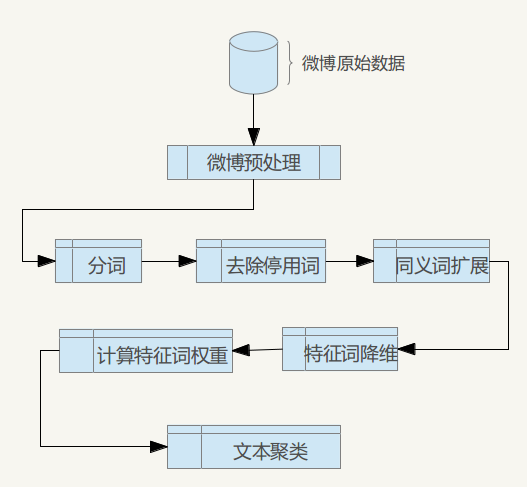
\includegraphics[width=1\textwidth,keepaspectratio]{weibo-mining-procedure.png}
    \column{0.45\textwidth}
    \pause
    \begin{tiny}
    \begin{itemize}
    \item<2- | alert@2> {微博预处理过程主要是由于原始的微博数据是~TREC~格式,
      微博文本中混有~XML~非法字符,如$<$,$>$, $\&$等,预处理过程将其去除,
      转换成~XML~标准格式。}
    
    \item<3-|alert@3> {分词采用计算所~ICTCLAS~分词程序的~Java~版本,由于原始的词
      库有限,为了达到最大的分词准确率,针对微博内容口语化的特点,我们新增了用户
      词典(搜狗输入法词库),主要是网络流行词汇,如``有木有'',``伤不起'',``高帅富''等新鲜词汇。}
    
    \item<4-|alert@4> {同义词扩展主要参考了《同义词词林》,以及其他网络同义词。}

    \item<5-|alert@5> {特征词降维主要是为了在保证聚类效果的情况下尽量减少聚类空
      间的维数,采用信息增益的方法进行降维,可以从信息论的观点最大可能保证原有信
      息流失尽可能少。}
    \item<6-|alert@6>{特征词权重计算采用了多种权重计算方法,如传统的~TF-IDF~,
      Okapi权重,TFC,熵权重,最终综合比较各种权重计算方法效果。}
    \item<7-|alert@7>{聚类采用Mahout程序库,由于该库包含了多种聚类
      方法,所以最终也可以比较不同聚类算法下的微博文本的聚类效果。}

    \end{itemize}
    \end{tiny}
  \end{columns}
\end{frame}

%%%%%%%%%%% 系统实现 %%%%%%%%%%%%%%
\section{系统实现}

\subsection{微博分词}
\begin{frame}[fragile]
  \frametitle{微博分词}
  \lstset{language=Java,basicstyle=\ttfamily,commentstyle=\ttfamily}
  \lstdefinestyle{Java}{delim=[il][\bfseries]{BB}}
  \definecolor{lightgray}{rgb}{.9,.9,.9}
  \lstset{backgroundcolor=\color{lightgray}}
  \begin{tiny}
    \begin{block}{}
      \begin{lstlisting}[language=Java]
        public String weiboSplitProcessing(String input) {
            try {
                byte nativeBytes[] = ictclas50.ICTCLAS_ParagraphProcess(
                    input.getBytes("GB2312"), 2, 0);
                String nativeStr = new String(nativeBytes, 0,
                    nativeBytes.length, "GB2312");
                return nativeStr;
            } catch (Exception e) {
            logger.debug(e.getMessage());
            return null;
            }
        }
    \end{lstlisting}
    \end{block}
  \end{tiny}
\end{frame}

% \begin{frame}[fragile]
%   \frametitle{微博分词}
%   \lstset{language=Java,basicstyle=\ttfamily,commentstyle=\ttfamily}
%   \lstdefinestyle{Java}{delim=[il][\bfseries]{BB}}
%   \definecolor{lightgray}{rgb}{.9,.9,.9}
%   \lstset{backgroundcolor=\color{lightgray}}
%   \begin{tiny}
%     \begin{block}{}
%       \begin{lstlisting}[language=Java]
%         public String weiboSplitProcessing(String input) {
%             try {
%                 byte nativeBytes[] = ictclas50.ICTCLAS_ParagraphProcess(
%                     input.getBytes("GB2312"), 2, 0);
%                 String nativeStr = new String(nativeBytes, 0,
%                     nativeBytes.length, "GB2312");
%                 return nativeStr;
%             } catch (Exception e) {
%             logger.debug(e.getMessage());
%             return null;
%             }
%         }
%     \end{lstlisting}
%     \end{block}
%   \end{tiny}
% \end{frame}

\begin{frame}[fragile]
  \frametitle{微博分词}
  \lstset{language=Java,basicstyle=\ttfamily,commentstyle=\ttfamily}
  \lstdefinestyle{Java}{delim=[il][\bfseries]{BB}}
  \definecolor{lightgray}{rgb}{.9,.9,.9}
  \lstset{backgroundcolor=\color{lightgray}}
  \begin{tiny}
    \begin{block}{}
      \begin{lstlisting}[language=Java]
    public class WeiboSplitter {
	    /**
	     * logger.
	     */
	    public static final Logger logger = 
            LoggerFactory.getLogger(WeiboSplitter.class);
        ICTCLAS50 ictclas50 = new ICTCLAS50();
        public WeiboSplitter() {
            super();
            try {
                if (ictclas50.ICTCLAS_Init(path.getBytes("GB2312")) == false) {
                    logger.debug("Init Failed!");
                }
            } catch (UnsupportedEncodingException e) {
                logger.debug(e.getMessage());
                e.printStackTrace();
            }
            ictclas50.ICTCLAS_SetPOSmap(2);
            byte[] usrdirb = usrdir.getBytes();
            int userDictsCounter = ictclas50.ICTCLAS_ImportUserDictFile(usrdirb, 0);
        }
        public String weiboSplitProcessing(String input) {
                        . . . . . .
        }
        public void finalize() {
            ictclas50.ICTCLAS_SaveTheUsrDic();
            ictclas50.ICTCLAS_Exit();
        }
    }
      \end{lstlisting}
    \end{block}
  \end{tiny}
\end{frame}

\subsection{去除停用词}
\begin{frame}[fragile]
  \frametitle{去除停用词}
  \lstset{language=Java,basicstyle=\ttfamily,commentstyle=\ttfamily}
  \lstdefinestyle{Java}{delim=[il][\bfseries]{BB}}
  \definecolor{lightgray}{rgb}{.9,.9,.9}
  \lstset{backgroundcolor=\color{lightgray}}
  \begin{tiny}
    \begin{block}{}
      \begin{lstlisting}[language=Java]
    public String remove(String sentence) {
        String regex = " ";
        String[] words = sentence.split(regex);
        StringBuilder stopWordRemoved = new StringBuilder();
        for (int i = 0; i < words.length; i++) {
        if (contains(words[i]));
            else {
                stopWordRemoved.append(words[i]);
                stopWordRemoved.append(" ");
            }
        }
        return stopWordRemoved.toString();
    }
      \end{lstlisting}
    \end{block}
  \end{tiny}
\end{frame}

\subsection{特征信息扩展}
\begin{frame}
  \frametitle{特征信息扩展}
  \begin{block}{}
    特征信息扩展初步选择同义词扩展。
  \end{block}
  \begin{block}{}
   采集的同义词库达到了10万数量级以上,《同义词词林》等。
  \end{block}
  \begin{block}{}
    还可以采用《知网》语言知识库。
  \end{block}
\end{frame}

\begin{frame}[fragile]
  \frametitle{特征信息扩展}
  \lstset{language=Java,basicstyle=\ttfamily,commentstyle=\ttfamily}
  \lstdefinestyle{Java}{delim=[il][\bfseries]{BB}}
  \definecolor{lightgray}{rgb}{.9,.9,.9}
  \lstset{backgroundcolor=\color{lightgray}}
  \begin{tiny}
    \begin{block}{}
      \begin{lstlisting}[language=Java]
    public String extendSynonymWords(String sentence) {
        String regex = " ";
        String[] words = sentence.split(regex);
        StringBuilder synonymWordsAdded = new StringBuilder();
        for (int i = 0; i < words.length; i++) {
            if (contains(words[i])) {
                synonymWordsAdded.append(words[i]);
                synonymWordsAdded.append(" ");
                synonymWordsAdded.append(synonymWords(words[i]));
            } else {
                synonymWordsAdded.append(words[i]);
                synonymWordsAdded.append(" ");
            }
        }
        return synonymWordsAdded.toString();
    }
    
    public String extendSynonymWords(String sentence, int depth) {
        if (depth <= 0) return sentence;
        else return extendSynonymWords(extendSynonymWords(sentence, depth - 1));
    }
      \end{lstlisting}
    \end{block}
  \end{tiny}
\end{frame}

\subsection{特征信息降维}
\begin{frame}
  \frametitle{特征信息降维}
  \begin{block}{特征词的选择}
    由于对微博内容先验知识的缺乏,本系统采取了词频与信息增益相结合的方式来进行
    特征信息的降维,特征信息增益越大,说明特征中包含的鉴别信息就越多,
    选择信息增益值的前50\%作为微博的特征向量。
  \end{block}

  \pause
  \begin{block}{词项$T_k$的信息增益IG}
    \pause
    \begin{small}
    \begin{eqnarray*}
      \begin{array}{crl}
        IG(T, T_k) &=&I(T) - I(T, T_k)\\
        &=& \sum_{k = 1 \cdots n}P_k \times \log P_k -
        \sum_{k = 1 \cdots n} \frac{P_k}{P_k \times \log P_k} \times P_k \times log P_k\\
      \end{array}
    \end{eqnarray*}
    \end{small}
  \end{block}
 
\end{frame}
\subsection{建立倒排索引}
\begin{frame}[fragile]
  \frametitle{建立倒排索引}
  \lstset{language=Java,basicstyle=\ttfamily,commentstyle=\ttfamily}
  \lstdefinestyle{Java}{delim=[il][\bfseries]{BB}}
  \definecolor{lightgray}{rgb}{.9,.9,.9}
  \lstset{backgroundcolor=\color{lightgray}}
\begin{tikzpicture}[scale=.5, transform shape]
  \tikzstyle{every node}=[draw,shape=rectangle];
  \node (TermM) at (0, 0) {词项m};
  \node (Term6) at (0, 1) {词项6};
  \node (Term5) at (0, 2) {词项5};
  \node (Term4) at (0, 3) {词项4};
  \node (Term3) at (0, 4) {词项3};
  \node (Term2) at (0, 5) {词项2};
  \node (Term1) at (0, 6) {词项1};

  \pause
  \node (WeiboPair71) at (3, 6) {$<$微博1,次数$>$};
  \node (WeiboPair72) at (7, 6) {$<$微博2,次数$>$};
  \node (WeiboPair73) at (11, 6) {$<$微博3,次数$>$};
  \node (WeiboPair74) at (15, 6) {$<$微博4,次数$>$};
  \node (WeiboPair7n) at (19, 6) {$<$微博n,次数$>$};

  \pause
  \node (WeiboPair61) at (3, 5) {$<$微博1,次数$>$};
  \node (WeiboPair62) at (7, 5) {$<$微博2,次数$>$};
  \node (WeiboPair63) at (11, 5) {$<$微博3,次数$>$};
  \node (WeiboPair64) at (15, 5) {$<$微博4,次数$>$};
  \node (WeiboPair6n) at (19, 5) {$<$微博n,次数$>$};

  \pause
  \node (WeiboPair51) at (3, 4) {$<$微博1,次数$>$};
  \node (WeiboPair52) at (7, 4) {$<$微博2,次数$>$};
  \node (WeiboPair53) at (11, 4) {$<$微博3,次数$>$};
  \node (WeiboPair54) at (15, 4) {$<$微博4,次数$>$};
  \node (WeiboPair5n) at (19, 4) {$<$微博n,次数$>$};

  \pause
  \node (WeiboPair41) at (3, 3) {$<$微博1,次数$>$};
  \node (WeiboPair42) at (7, 3) {$<$微博2,次数$>$};
  \node (WeiboPair43) at (11, 3) {$<$微博3,次数$>$};
  \node (WeiboPair44) at (15, 3) {$<$微博4,次数$>$};
  \node (WeiboPair4n) at (19, 3) {$<$微博n,次数$>$};

  \pause
  \node (WeiboPair31) at (3, 2) {$<$微博1,次数$>$};
  \node (WeiboPair32) at (7, 2) {$<$微博2,次数$>$};
  \node (WeiboPair33) at (11, 2) {$<$微博3,次数$>$};
  \node (WeiboPair34) at (15, 2) {$<$微博4,次数$>$};
  \node (WeiboPair3n) at (19, 2) {$<$微博n,次数$>$};

  \pause
  \node (WeiboPair21) at (3, 1) {$<$微博1,次数$>$};
  \node (WeiboPair22) at (7, 1) {$<$微博2,次数$>$};
  \node (WeiboPair23) at (11, 1) {$<$微博3,次数$>$};
  \node (WeiboPair24) at (15, 1) {$<$微博4,次数$>$};
  \node (WeiboPair2n) at (19, 1) {$<$微博n,次数$>$};

  \pause
  \node (WeiboPair11) at (3, 0) {$<$微博1,次数$>$};
  \node (WeiboPair12) at (7, 0) {$<$微博2,次数$>$};
  \node (WeiboPair13) at (11, 0) {$<$微博3,次数$>$};
  \node (WeiboPair14) at (15, 0) {$<$微博4,次数$>$};
  \node (WeiboPair1n) at (19, 0) {$<$微博n,次数$>$};

  \pause
  \foreach \from/\to in {TermM/WeiboPair11, WeiboPair11/WeiboPair12,
  WeiboPair12/WeiboPair13, WeiboPair13/WeiboPair14, WeiboPair14/WeiboPair1n}
  \draw[->] (\from) -- (\to);

  \foreach \from/\to in {TermM/WeiboPair11, WeiboPair11/WeiboPair12,
  WeiboPair12/WeiboPair13, WeiboPair13/WeiboPair14, WeiboPair14/WeiboPair1n}
  \draw[->] (\from) -- (\to);

  \foreach \from/\to in {Term6/WeiboPair21, WeiboPair21/WeiboPair22,
  WeiboPair22/WeiboPair23, WeiboPair23/WeiboPair24, WeiboPair24/WeiboPair2n}
  \draw[->] (\from) -- (\to);

  \foreach \from/\to in {Term5/WeiboPair31, WeiboPair31/WeiboPair32,
  WeiboPair32/WeiboPair33, WeiboPair33/WeiboPair34, WeiboPair34/WeiboPair3n}
  \draw[->] (\from) -- (\to);

  \foreach \from/\to in {Term4/WeiboPair41, WeiboPair41/WeiboPair42,
  WeiboPair42/WeiboPair43, WeiboPair43/WeiboPair44, WeiboPair44/WeiboPair4n}
  \draw[->] (\from) -- (\to);

  \foreach \from/\to in {Term3/WeiboPair51, WeiboPair51/WeiboPair52,
  WeiboPair52/WeiboPair53, WeiboPair53/WeiboPair54, WeiboPair54/WeiboPair5n}
  \draw[->] (\from) -- (\to);

  \foreach \from/\to in {Term2/WeiboPair61, WeiboPair61/WeiboPair62,
  WeiboPair62/WeiboPair63, WeiboPair63/WeiboPair64, WeiboPair64/WeiboPair6n}
  \draw[->] (\from) -- (\to);

  \foreach \from/\to in {Term1/WeiboPair71, WeiboPair71/WeiboPair72,
  WeiboPair72/WeiboPair73, WeiboPair73/WeiboPair74, WeiboPair74/WeiboPair7n}
  \draw[->] (\from) -- (\to);
\end{tikzpicture}
\end{frame}

\subsection{特征词权重计算}
\begin{frame}
  \frametitle{特征词权重计算}
  \begin{tiny}
    \begin{block}{}
      \begin{itemize}
        \item<1- | alert@1>{Okapi权重\cite{Robertson}
          $$
          w(t, D) = \ln \frac{N-df+0.5}{df + 0.5}\cdot
          \frac{(k_1 + 1) tf}{(k_1(1-b)+b\frac{L_D}{E(D)})+tf}
          $$}
        \item<2- | alert@2>{TFC
          $$
          w(t, D) = \frac{\log (tf + 1.0) \times \log \frac{N}{df}}{\sqrt{\sum_{t \in
          D}\left[\log (tf + 1.0) \times \log \frac{N}{df}\right]^2}}
          $$}
        \item<3- | alert@3>{熵权重
          $$
          w(t, D) = \log (tf + 1.0) \times \left (1 + \frac{1}{\log N} \times
          \sum_{j = 1}^N\left [\frac{tf_j}{df} \times \log
          \frac{tf_j}{df}\right]\right)
          $$}
        \item<4- | alert@4>{Pivoted Normalization 权重\cite{Singhal}
          $$
          w(t, D) = \sum_{t\in D} \frac{1 + \ln (1+ \ln(tf))}{(1-s)+s
          \frac{L_D}{E(D)}}\cdot \ln \frac{N+1}{df}
          $$}
        \end{itemize}
    \end{block}
  \end{tiny}
\end{frame}

\begin{frame}[fragile]
  \frametitle{特征词权重计算}
  \lstset{language=Java,basicstyle=\ttfamily,commentstyle=\ttfamily}
  \lstdefinestyle{Java}{delim=[il][\bfseries]{BB}}
  \definecolor{lightgray}{rgb}{.9,.9,.9}
  \lstset{backgroundcolor=\color{lightgray}}
  \begin{tiny}
    \begin{block}{}
      \begin{lstlisting}[language=Java]
    public Map<String, Map<String, Double>> weight(WeiboXMLHandler.Weibo weibo) {
        String docNo = weibo.getDocNo();
        Map<String, Map<String, Double>> mapWeight = new HashMap<String, Map<String,Double>>();
        Map<String, Double> mapTermWeight = new TreeMap<String, Double>();
        Iterator iterSetUniqueTerms = setUniqueTerms.iterator();
        while (iterSetUniqueTerms.hasNext()) {
            String term = (String) iterSetUniqueTerms.next();
            double weight = calculateTermWeight(term, weibo);
            mapTermWeight.put(term, new Double(weight));
        }
        mapWeight.put(docNo, mapTermWeight);
        return mapWeight;
    }
      \end{lstlisting}
    \end{block}
  \end{tiny}
  \pause
  \begin{tiny}
    \begin{block}{}
      返回值(微博ID : $<$特征词1, 权重1$>$ $<$特征词2, 权重2$>$ ...$<$特征词n, 权重n$>$)
    \end{block}
  \end{tiny}
\end{frame}

\subsection{聚类}
\begin{frame}
  \frametitle{聚类}
  \begin{block}{}
    聚类采用Mahout库中的工具进行聚类。
  \end{block}
  \pause
  \begin{block}{}
    The Apache \href{http://mahout.apache.org/}{$Mahout^{TM}$} machine learning library's goal is to build scalable
    machine learning libraries\cite{Mahout}, which provides:
    \begin{center}
    \begin{itemize}
        \item Collaborative Filtering
        \item User and Item based recommenders
        \item K-Means, Fuzzy K-Means clustering
        \item Mean Shift clustering
        \item Dirichlet process clustering
        \item Latent Dirichlet Allocation
        \item And much much more\ldots
      \end{itemize}
    \end{center}
  \end{block}
  
\end{frame}

%%%%%%%%%%% 测试与结论 %%%%%%%%%%%%%%
\section{测试与结论}
\begin{frame}
  \frametitle{测试与结论}
\end{frame}

\section{参考文献}
\begin{frame}
  \frametitle{参考文献}
  \begin{tiny}
  \begin{thebibliography}{99}
    \bibitem[Yu Hong, 2006]{Yu Hong}{洪宇,张宇,刘挺,李生,话题检测与跟踪的评测及研究综述,2006}
    \bibitem[Shi Jing, 2009]{Shi}{SHI Jing, FAN Meng, LI Wan-Long, 
      Topic Analysis Based on LDA Model, Acta Automatica Sinica, vol.35(12),
      pp.1586-1592, 2009}
    \bibitem[Rong Lu]{Rong}{Rong Lu, Liang Xiang, M.R. Liu, Qing Yang, Extracting News Topics from Microblogs based on Hidden Topics Analysis and Text Clustering}
    \bibitem[Wang Wei]{Wang}{王伟,许鑫,基于聚类的网络舆情热点发现及分析,情报分析与研究,2009}
    \bibitem[Tang, 2011]{Tang}{汤寒青,王汉军,改进的 K-means 算法在网络舆情分析中的应用,计算机系统应用,2011年~第20卷~第3期}
    \bibitem[Li Heng-Xun,2009]{Li}{李恒训,张华平,秦鹏,于满泉,刘金刚,基于主题词的网络热点话题发现,2009}
    \bibitem[Wikipedia,文本信息检索]{Wikipedia-IR}http://zh.wikipedia.org/zh/文本信息检索
    \bibitem[Salton,1975]{Salton}G. Salton, A. Wong, and C.S. Yang, ``A
      vector space model for information retrieval'', Communications of the ACM,
      vol. 18(11), pp. 613–620, 1975.
    \bibitem[Robertson, 1999]{Robertson}S. E. Robertson, S. Walker, and M.
      Beaulieu, ``Okapi at TREC7, automatic ad hoc, filtering, VLC and filtering
      tracks'', in Seventh Text REtrieval Conference (TREC-7), pp. 253–264, 1999.
    \bibitem[Singhal, 1999]{Singhal}A. Singhal, J. Choi, D. Hindle, D. Lewis,
      and F. Pereira, ``AT\&Tat TREC 7'', in Proceedings of the Seventh Text
      REtrieval Conference(TREC-7), vol. 500, pp. 239–252, 1999.
    \bibitem[Mahout, official website]{Mahout}http://mahout.apache.org/
  \end{thebibliography}
  \end{tiny}
\end{frame}

\end{CJK}
\end{document}
